
%----------------------------------------------------------------------------------------------------------------------
\begin{frame}{Proposed Methodology}
\begin{itemize}[noitemsep,label=\textbullet,topsep=2pt,parsep=2pt,partopsep=2pt]
\item To concurrently build mid-surfaces as part gets created (called forward create). 
\item At each feature step, shapes are relatively simple than final shape, thus creation of mid-surfaces at each stage is far simpler
\item For each feature, decide its contribution to Midsurface model
	\begin{itemize}[noitemsep,label=\textbullet,topsep=2pt,parsep=2pt,partopsep=2pt]
	\item 2D Profiles , generate Midcurves
	\item Primitives, generate predefined Midsurfaces
	\item Sweep based : Sweep Midcurves
	\item Boolean : Extend and Trim
	\end{itemize}
\end{itemize}
\end{frame}
%----------------------------------------------------------------------------------------------------------------------

\begin{frame}{What is so special about Feature Tree}
\begin{itemize}[noitemsep,label=\textbullet,topsep=2pt,parsep=2pt,partopsep=2pt]
\item Feature based Modeling is a powerful paradigm compared to modeling shapes by mesh or faces.
\item Feature is a geometrical shape characterized by attributes relevant to the domains
\item Part construction is stored as a sequence of features, in form of a Tree.
\item Parametric nature of the Features and Update mechanism, give powerful editing capabilities.
\item Most contemporary CAD packages use this to build and update models.
\end{itemize}
\end{frame}

%
%%----------------------------------------------------------------------------------------------------------------------
%\begin{frame}{System Architecture}
%\vspace{0.1cm}
%\centering 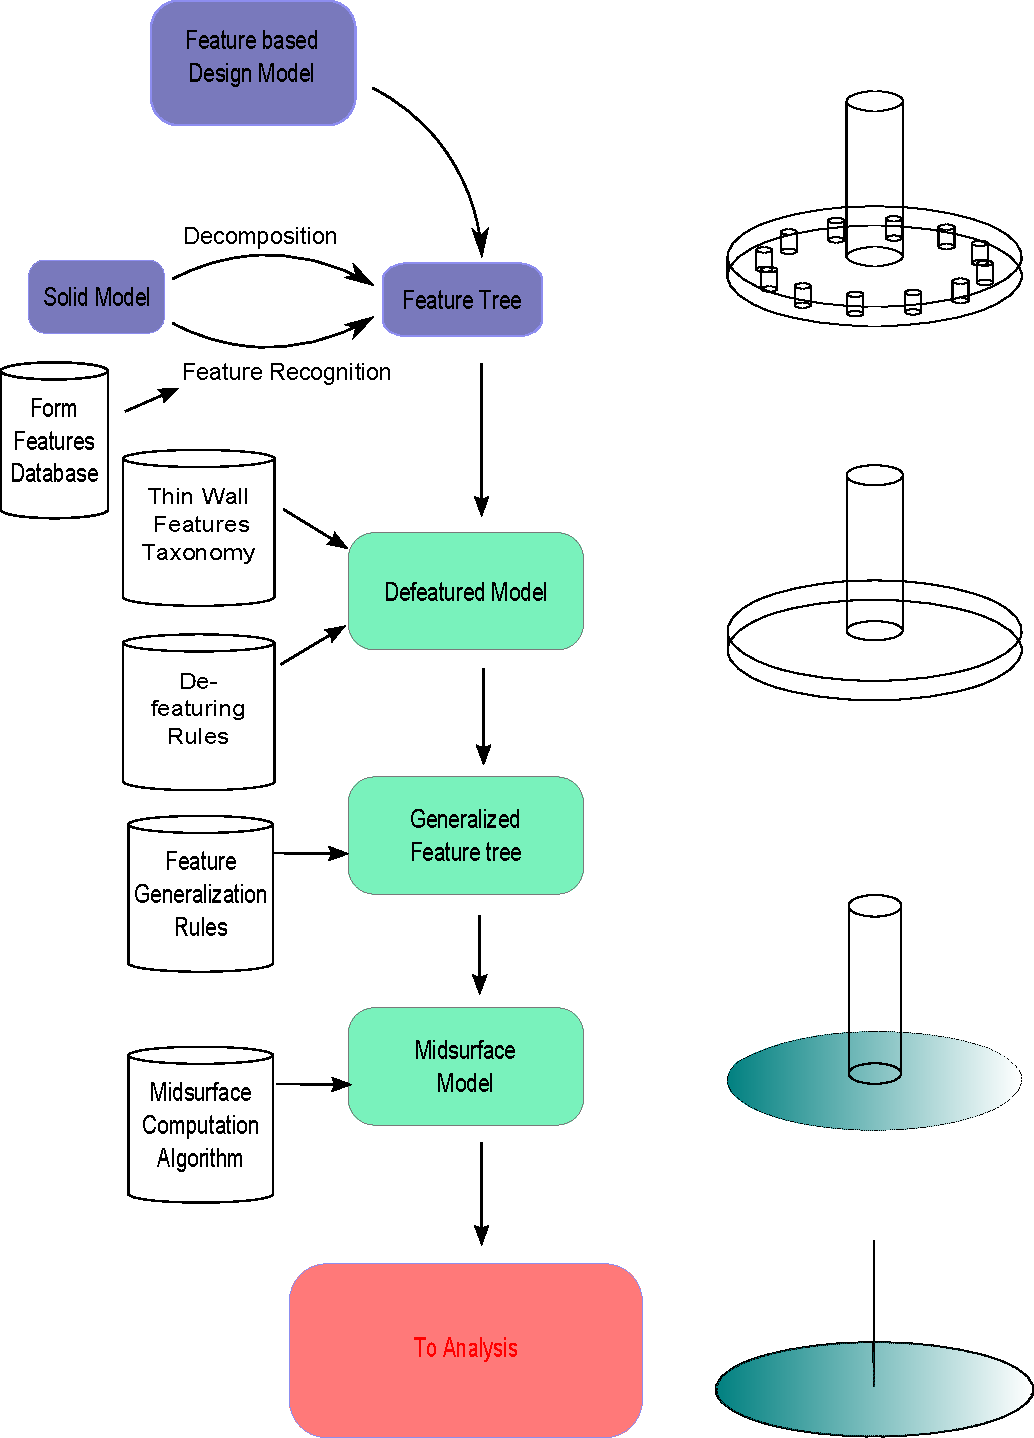
\includegraphics[height=0.7\linewidth]{../Common/images/SystemArchitecture.pdf}
%\end{frame}
%%----------------------------------------------------------------------------------------------------------------------


%----------------------------------------------------------------------------------------------------------------------

\begin{frame}[<+-| alert@+>]{Proposal}

\begin{itemize}[noitemsep,label=\textbullet,topsep=2pt,parsep=2pt,partopsep=2pt]
\item To concurrently build mid-surfaces as part gets created (called forward create). 
\item At each feature step, shapes are relatively simple than final shape, thus creation of mid-surfaces at each stage is far simpler.
\item After development of Boolean of non-manifold shapes, this method can build well connected, isomorphic mid-surfaces better than reverse engineer way, which is currently followed.
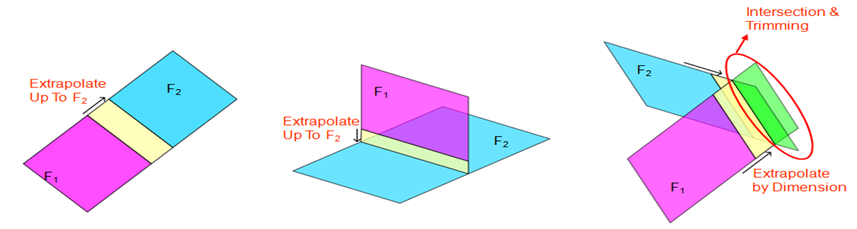
\includegraphics[scale=0.4]{../Common/images/ExtendTrim.png}

\end{itemize}
\end{frame}


%----------------------------------------------------------------------------------------------------------------------


\begin{frame}[<+-| alert@+>]{Overall Approach}

\begin{columns}[T]
\column{0.5\textwidth}

	\begin{itemize}[noitemsep,label=\textbullet,topsep=2pt,parsep=2pt,partopsep=2pt]
	\item De-featuring will suppress irrelevant features
	\item For each feature, decide its contribution to Midsurface model
	\begin{itemize}[noitemsep,label=\textbullet,topsep=2pt,parsep=2pt,partopsep=2pt]
	\item 2D Profiles , generate Midcurves
	\item Primitives, generate predefined Midsurfaces
	\item Sweep based : Sweep Midcurves
	\item Boolean : Extend and Trim
	\end{itemize}
	\end{itemize}

\column{0.5\textwidth}

	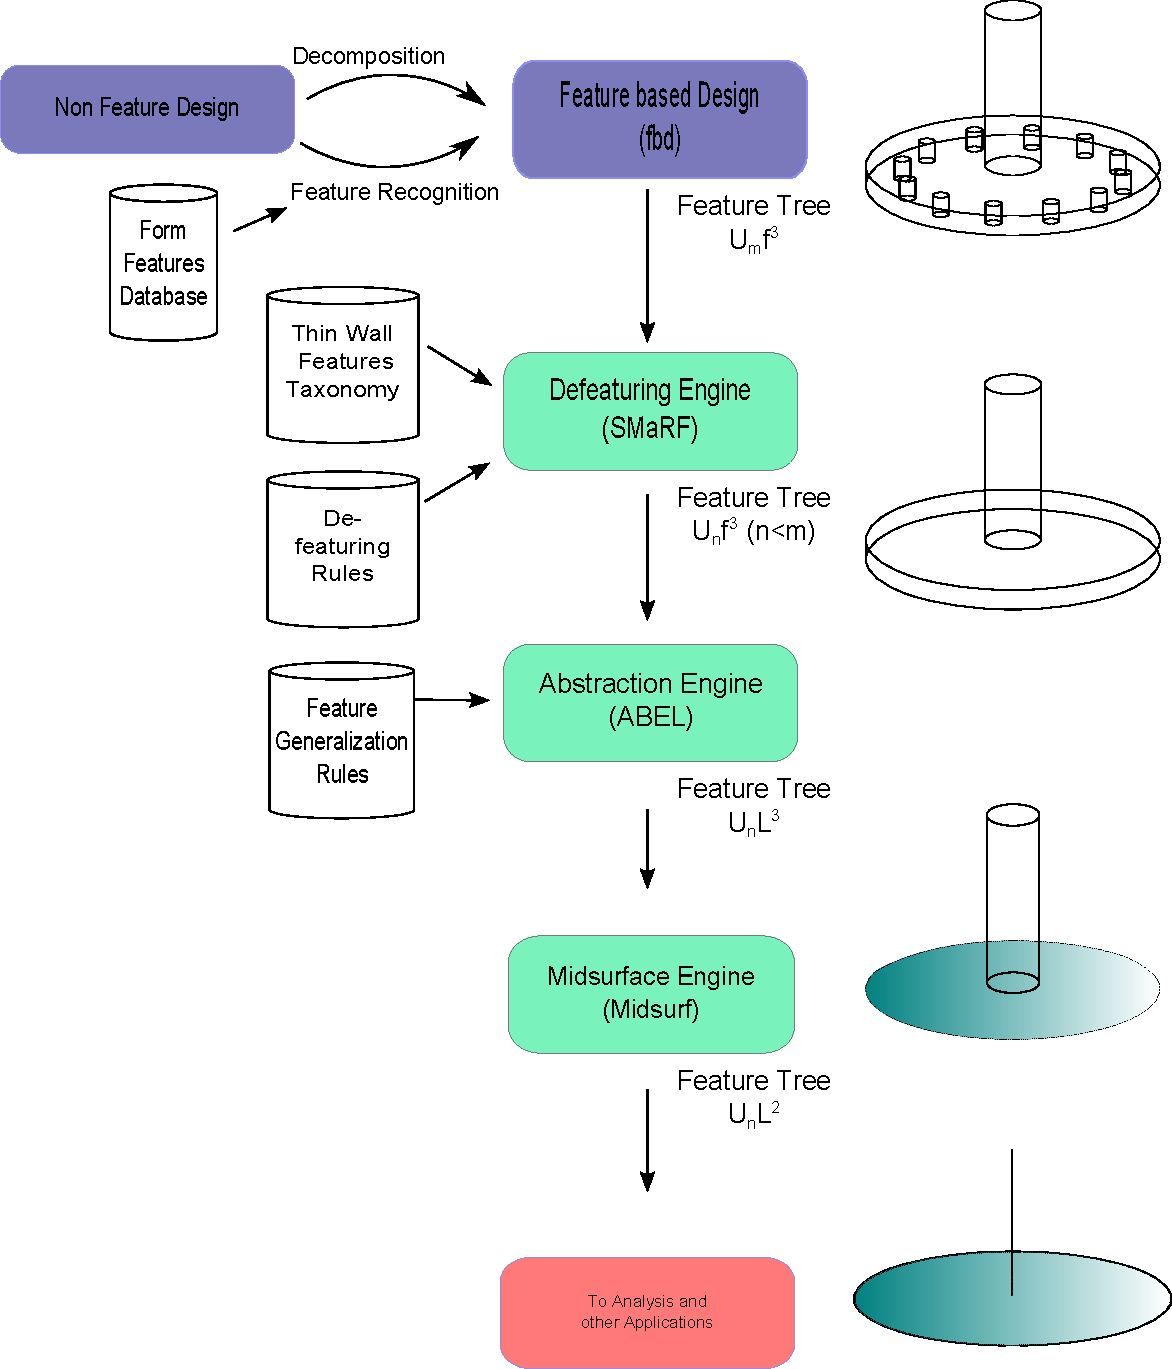
\includegraphics[scale=0.25]{../Common/images/SystemArchitecture1.pdf}

\end{columns}

\end{frame}
%%------------------------------------------------------------------------------------------------------------------------------------
%
%\begin{frame}[<+-| alert@+>]{De-featuring}
%
%\begin{itemize}[noitemsep,label=\textbullet,topsep=2pt,parsep=2pt,partopsep=2pt]
%\item Given a feature tree, compute simplified model by suppressing certain features
%\item Part Bounding Box, $x \%$ of Diagonal length
%\end{itemize}
%
%\begin{columns}
%\column{0.35\textwidth}
%	\vspace{-3.2cm}
%	\begin{tabular}[h]{@{} l l   @{}}
%	\toprule
%	{\bf Feature } & {\bf Comparison } \\
%	\midrule
%	Hole & Diameter \\
%	Fillet & Radius \\
%	Chamfer & Side \\
%	Primitives & Size \\
%	Patterns & Keep Master \\
%	\bottomrule
%	\end{tabular}
%\column{0.45\textwidth}
%	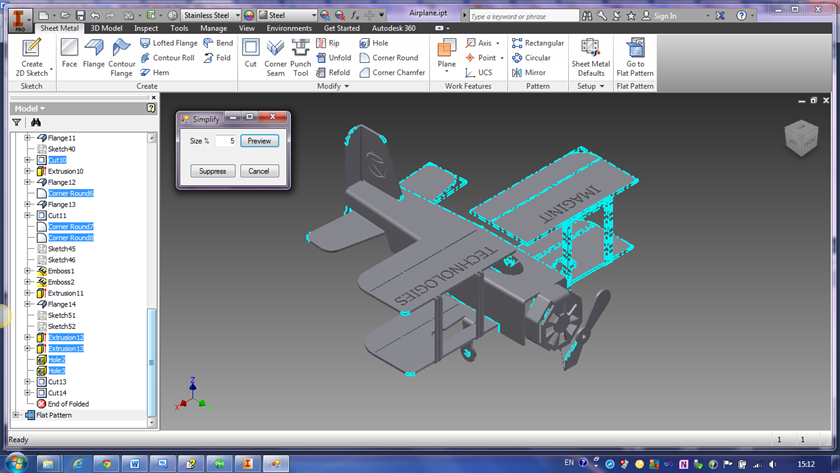
\includegraphics[scale=0.4]{../Common/images/Defeaturing.png}
%\end{columns}
%
%\end{frame}
%%------------------------------------------------------------------------------------------------------------------------------------
%
%\begin{frame}[<+-| alert@+>]{2D Midcurves}
%
%\begin{itemize}[noitemsep,label=\textbullet,topsep=2pt,parsep=2pt,partopsep=2pt]
%\item Given a 2D closed profile, get connected medial curves, no extra branches
%\item Decompose 2D to find its sub regions, like features in 3D. Sub regions being simpler, it would be easy to get Midcurves, than skeleton of whole Profile.
%\item Generate individual midcurves. Extend and Join
%	
%\vspace{1cm}
%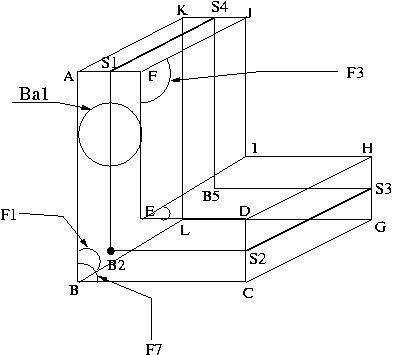
\includegraphics[scale=0.45]{../Common/images/Ramanathan.jpg}
%
%\end{itemize}
%
%
%\end{frame}
%------------------------------------------------------------------------------------------------------------------------------------

